%\documentclass[12pt]{article}
\documentclass{beamer}
\usetheme{Madrid}
\usecolortheme{seahorse}

\usepackage{fontspec}
\usepackage{polyglossia}
\setdefaultlanguage{english}

\usepackage{tikz}
\usetikzlibrary{calc}

\usepackage{color}
\usepackage{fancyvrb}

\usepackage{qrcode}

% https://tex.stackexchange.com/questions/16793/global-setting-of-spacing-between-items-in-itemize-environment-for-beamer
\let\olditem\item
\renewcommand{\item}{%
\olditem\vspace{4pt}}

\usepackage{amsthm}
\newtheorem{mydef}{Definition}

\newcommand{\bigO}[1]{\ensuremath{\mathcal{O}(#1)}}

%\usepackage{minted}

\usepackage[noend]{algpseudocode} % No explicit "end function" line
\newcommand*\AlgLet[2]{\State #1 $\gets$ #2} % X <- Y assignment

\title[SAT-based preimage attack optimizations]{Evaluation of SAT-based\\ preimage attack optimizations}
\author[Ladislav Pápay]{Ladislav Pápay\\~\\~\\ Supervisor: doc. RNDr. Martin Stanek PhD.}
\date{}

\begin{document}

\frame{\titlepage}

%%%% OUTLINE
%
% - title
% - problem overview - hash preimage
% - existing work / refs
% - goals + library
% - code sample / sha1 comparison
% - expression opt - example with choice fnc
% - sha1 comparison plot
% - gh analysis + sha3 results + conclusion
% - branching order - overview
% - sha3 comparison plot
% - gh analysis + conclusion
% - ? other opts / ...
% - summary
% - thanks  + questions? (+ doi/link)
%
%
% OLD
% - tseitin translation
% - existing
% - our approach (operator overloading,...), md5,sha1,sha3 done, easy to do more
% - comparison, simpler code
% - problems - (partial) preimage, (partial) collision
% - graphs
% - further experiments - branch order, ...
% - pros/cons - can prove some preimage doesnt exist (unlike bruteforce), much slower though, not parallelizable
% - conclusion/summary
% - questions/thanks

\begin{frame}
\frametitle{Problem introduction}
\begin{itemize}
\item \textbf{Hash function} $h: X \to Y$, usually $|X| \gg |Y|$
\begin{itemize}
	\item \emph{Easy} to compute $h(x)$ given $x$
	\item \emph{Hard} to find $x'$ such that $h(x') = y$ given $y$
	\begin{itemize}
		\item \textbf{Preimage attack}
	\end{itemize}
\end{itemize}
\item \textbf{SAT solvers} can find solutions to any boolean satisfiability problem
\begin{itemize}
	\item \emph{Instance} = variables and clauses in conjunctive normal form
\end{itemize}
\end{itemize}
\end{frame}

\begin{frame}
\frametitle{Using SAT for preimage attacks}
\begin{itemize}
\item \textbf{Idea:} model $h(x) = y$ as a SAT instance
\begin{itemize}
	\item Fix value of $y$ using additional constraints
	\item Let SAT solver find solution for $x$
\end{itemize}
\item First proposed in \emph{Logical cryptanalysis as a SAT problem} (Massacci, Marraro, 2000) on the \emph{DES} cipher
\item Other works focused on hash functions (\emph{MD4}, \emph{MD5}, \emph{SHA-1}, \dots)
\item \textbf{Problems}
\begin{itemize}
	\item Hand crafted specialized programs to generate instances
	\item Code not available
	\item Toolkit uses proprietary and niche technologies
\end{itemize}
\end{itemize}
\end{frame}

\begin{frame}
\frametitle{Our Approach}
\begin{itemize}
\item Python library that provides a custom data type \textit{BitVector}
\begin{itemize}
	\item Behaves in the same way as any integer type
	\item Using operator overloading creates the boolean circuit automatically
\end{itemize}
\item Model can be made with minimal changes to existing implementations of cryptographic primitives
\begin{itemize}
	\item So far implemented MD5, SHA-1 and SHA-3 (Keccak)
\end{itemize}
\item Saves time, less error-prone
\end{itemize}
\end{frame}

\begin{frame}[fragile]
\frametitle{Approach Comparison (SHA-1 round functions)}
\begin{minipage}[t]{.4\textwidth}
\textit{Vegard Nossum, 2012}
{\tiny
\begin{verbatim}
if (i >= 0 && i < 20) {
  for (unsigned int j = 0; j < 32; ++j) {
    clause(-f[j], -b[j], c[j]);
    clause(-f[j], b[j], d[j]);
    clause(-f[j], c[j], d[j]);

    clause(f[j], -b[j], -c[j]);
    clause(f[j], b[j], -d[j]);
    clause(f[j], -c[j], -d[j]);
  }
} else if (i >= 20 && i < 40) {
  xor3(f, b, c, d);
} else if (i >= 40 && i < 60) {
  for (unsigned int j = 0; j < 32; ++j) {
    clause(-f[j], b[j], c[j]);
    clause(-f[j], b[j], d[j]);
    clause(-f[j], c[j], d[j]);

    clause(f[j], -b[j], -c[j]);
    clause(f[j], -b[j], -d[j]);
    clause(f[j], -c[j], -d[j]);
  }
} else if (i >= 60 && i < 80) {
  xor3(f, b, c, d);
}
\end{verbatim}}
\end{minipage}
\hfill
\begin{minipage}[t]{.5\textwidth}
\textit{Our Approach}
{\tiny
\begin{verbatim}
if 0 <= i < 20:
  f = (b & c) | (~b & d)
elif 20 <= i < 40:
  f = b ^ c ^ d
elif 40 <= i < 60:
  f = (b & c) | (b & d) | (c & d)
else:
  f = b ^ c ^ d
\end{verbatim}}
\begin{itemize}
\item This is round function only
\item Overall $\approx$100 lines vs. $\approx$25 lines
\end{itemize}
\end{minipage}
\end{frame}

\begin{frame}
\frametitle{Cryptographic Problems}
\begin{itemize}
\item The model generated for some cryptographic primitive can be easily further constrained
\item Examples for hash functions
\begin{itemize}
\item (Partial) Preimage attack
\begin{itemize}
\item Any number of output bits can be set to either \textit{1} or \textit{0}
\item Satisfiable model assignment provides input message with desired hash image
\item Unsatisfiable model means no such message exists
\end{itemize}
\item (Partial) Collision
\begin{itemize}
\item Taking two hash function models with non-identical inputs but with any number of output bits equal
\item Satisfiable model assignment provides two different input messages with hash images that match on specified bits
\end{itemize}
\end{itemize}
\end{itemize}
\end{frame}

\begin{frame}[fragile]
\frametitle{Example of use -- HashToolkit}
\begin{Verbatim}[commandchars=\\\{\}]
$ python3 hashtoolkit.py -h sha1 -l 64 -o '{\color{red}00001111}'
Setting variables...
Generating clauses...
==================[ Problem Statistics ]===================
|  Number of variables:         43232                     |
|  Number of clauses:          175437                     |
===========================================================
conflicts   : 1170       (923 /sec)
decisions   : 27318      (0.00 % random) (21544 /sec)
CPU time    : 1.268 s

SATISFIABLE

Message bytes: b'{\color{red}YZ[o_DtQ}' rounds:  80
sha1 {\color{red}0f}083bf74420893176930c9ffc90e946d91c9fb7
\end{Verbatim}
\end{frame}
%$ % fix syntax highlighting

\begin{frame}
\frametitle{Tseitin transformation}
\begin{itemize}
\item Expressions are converted to a \emph{boolean circuit} and then to clauses
\begin{itemize}
	\item Uses additional variables to avoid exponential size of output
\end{itemize}
\item For example, \texttt{X = A \& (B \^{} C)}
\end{itemize}
\begin{center}
\resizebox{0.75\textwidth}{!}{
  \begin{tikzpicture}[every node/.style = {draw, shape=rectangle, inner sep=2mm,
                                  font=\fontsize{22}{25}\selectfont},
             every tree node/.style={}, level distance=25mm, sibling distance=30mm]
\node (and) {$\land$} [grow = up]
  child {node (xor) {$\oplus$}
    child {node [shape=circle, inner sep=1mm] {C}}
    child {node [shape=circle, inner sep=1mm] {B}}
  }
  child {node [shape=circle, inner sep=1mm] {A}};

\node at (and.south east) [xshift=4mm, draw=none] {\small X};
\node at (xor.south east) [xshift=4mm, draw=none] {\small Y};

\node (arrstart) at (xor.east) [xshift=15mm, draw=none] {};
\node (arrend) at (xor.east) [xshift=30mm, draw=none] {};
\draw [->, line width=2pt] (arrstart) -- (arrend);

\node [right of=arrend, draw=none, inner sep=1mm, text width=45mm, xshift=25mm, yshift=13mm] {$(Y \lor B \lor \overline{C}) \land (Y \lor \overline{B} \lor C) \land (\overline{Y} \lor B \lor C) \land (\overline{Y} \lor \overline{B} \lor \overline{C})~\land$};
\node [right of=arrend, draw=none, inner sep=1mm, text width=45mm, xshift=25mm, yshift=-22mm] {$ (X \lor \overline{A} \lor \overline{Y}) \land (\overline{X} \lor A) \land (\overline{X} \lor Y)$};

\node (arr2start) at (xor.east) [xshift=95mm, draw=none] {};
\node (arr2end) at (xor.east) [xshift=110mm, draw=none] {};
\draw [->, line width=2pt] (arr2start) -- (arr2end);


\node [right of=arr2end, draw=none, text width=40mm, xshift=20mm] {\texttt{4 2 -3 0\\4 -2 3 0\\-4 2 3 0\\-4 -2 -3 0\\~\\5 -1 -4 0\\-5 1 0\\-5 4 0}};

\end{tikzpicture}
% 1=A, 2=B, 3=C, 4=Y, 5=X
%%%%
%2 3 -4 0
%2 -3 4 0
%-2 3 4 0
%-2 -3 -4 0
%-5 1 0
%-5 4 0
%5 -1 -4 0

}
\end{center}
\begin{itemize}
\item Possible problem: automatic and transparent conversion of expressions to SAT instance might not be optimal
\end{itemize}
\end{frame}

\begin{frame}
\frametitle{Expression optimization}
Choice function in \emph{SHA-1}: $Ch(x, y, z) = (x \land y) \oplus (\overline{x} \land z)$
%\vspace{20pt}
\vfill
\begin{minipage}[t][][t]{.35\textwidth}
\emph{Tseitin transformation}\\(Automatic)
{\small \begin{align*}
(\overline{a} \lor x), (\overline{a} \lor y), (a \lor \overline{x} \lor \overline{y}) \\
(\overline{b} \lor \overline{x}), (\overline{b} \lor z), (b \lor x \lor \overline{z})\\
(c \lor a \lor \overline{b}), (c \lor \overline{a} \lor b) \\
(\overline{c} \lor a \lor b), (\overline{c} \lor \overline{a} \lor \overline{b})
\end{align*}}%
\end{minipage}
\begin{minipage}[t][][t]{.3\textwidth}
\emph{Hand conversion}\\(Nossum, 2012)
{\small \begin{align*}
(\overline{a} \lor \overline{x} \lor y), (\overline{a} \lor x \lor z) \\
(\overline{a} \lor y \lor z), (a \lor \overline{x} \lor \overline{y}) \\
(a \lor x \lor \overline{z}), (a \lor \overline{y} \lor \overline{z})
\end{align*}}%
\end{minipage}
\begin{minipage}[t][][t]{.25\textwidth}
\emph{Espresso} heuristic logic minimizer
{\small \begin{align*}
(a \lor \overline{x} \lor \overline{y}), (a \lor x \lor \overline{z})\\
(\overline{a} \lor x \lor z), (\overline{a} \lor \overline{x} \lor y)
\end{align*}}%
\end{minipage}
\begin{minipage}[b][][b]{0.35\textwidth}
10 clauses\\
3 additional variables\end{minipage}
\begin{minipage}[b][][b]{0.3\textwidth}
6 clauses\\
1 variable
\end{minipage}
\begin{minipage}[b][][b]{0.25\textwidth}
4 clauses\\
1 variable
\end{minipage}
\end{frame}

\begin{frame}
\begin{itemize}
\item Added expression optimization using \emph{Espresso} to our library
\end{itemize}
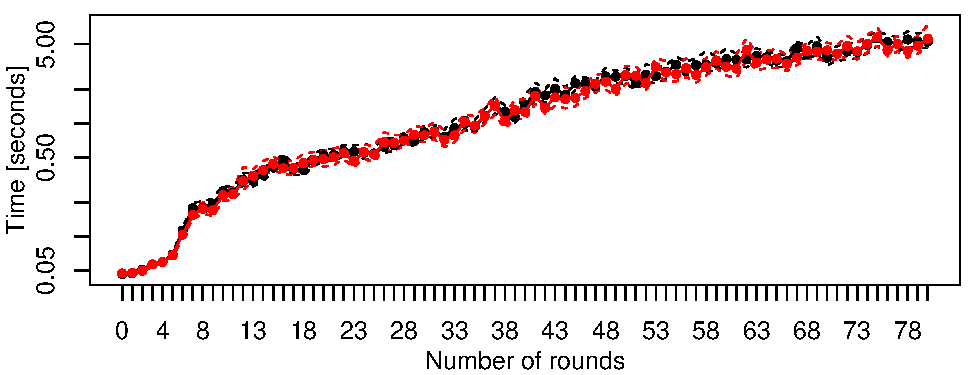
\includegraphics[width=\textwidth]{figures/opt-sha1/sha1-32bit-8bitref-cmp-espresso.pdf}
\begin{itemize}
\item Reduces number of variables and clauses, but not solving time
\begin{itemize}
	\item No need to use it, minimal changes to existing implementations
\end{itemize}
\end{itemize}
\end{frame}

\begin{frame}
TODO branch ordering
\end{frame}

\begin{frame}
\frametitle{Conclusions}
TODO
\end{frame}

\begin{frame}
\centering
{\Huge Thank you!}\\
~\\
{\Huge Questions?}\\
\vspace{30pt}
Library, usage examples and more available at:\\
\vspace{20pt}
\begin{minipage}{.3\textwidth}
http://dx.doi.org/10.5281/zenodo.48832
\end{minipage}
\hspace{100pt}
\begin{minipage}{.3\textwidth}
\qrcode[height=3cm]{http://dx.doi.org/10.5281/zenodo.48832}
\end{minipage}
\end{frame}

\end{document}
